\chapter{Planteamiento del Problema}
\noindent En este capítulo se hablará de que es el Instituto Politécnico Nacional, como esta conformada, las actividades deportivas que en está se practican, así como los problemas que se tienen en estos úlitmos.
Con esto se presentará softwares que existen en el mercado que pueden ayudar a mitigar parte de los problemas existentes, sin embargo, como se mostrará no cubren en su totalidad los problemas existentas siendo así se presenta la solución propuesta por alumnos de la Escuela Superior de Cómputo.

%=========================================================
%                                                         Justificacion
%=========================================================
\section{Antecedentes}
\noindent El Instituto Politécnico Nacional (IPN) es una institución educativa del Estado creada para consolidar, a través de la educación, la Independencia Económica, Científica, Tecnológica, Cultural y Política para alcanzar el progreso social de la Nación, de acuerdo con los objetivos Históricos de la Revolución Mexicana, contenidos en la Constitución Política de los Estados Unidos Mexicanos.
\noindent En 1932 surgió la idea de integrar y estructurar un sistema de enseñanza técnica, proyecto en el cual participaron destacadamente el licenciado Narciso Bassols y los ingenieros Luis Enrique Erro y Carlos Vallejo Márquez.
\noindent Sus fundadores concibieron al Politécnico como un motor de desarrollo y espacio para la igualdad; apoyando por una parte, el proceso de industrialización del país y, por la otra, brindando alternativas educativas a todos los sectores sociales, en especial a los menos favorecidos​\cite{ipnMision}.
\noindent Actualmente el IPN está conformado por 46 Unidades Académica, considerando solo el Nivel Medio Superior y Nivel Superior. En cada una de ellas, además de seguir el plan de estudios correspondientes, se llevan a cabo distintas actividades deportivas con la finalidad de fomentar en los alumnos una mejor calidad de vida, así como el alejar a estos del consumo de drogas entre otros. \\
\noindent Se han creado eventos que fomentan la participación y competitividad de la comunidad, llamados interpolitécnicos. Estos involucran áreas tales como: actividades deportivas, culturales o académicas, dichos eventos son de participación gratuita y se realizan 2 veces al año entre todos los planteles académicos que constituyen al IPN, divididas en los niveles Medio Superior y Superior.  \cite{Reglas}\\
\noindent El IPN cuenta con 26 actividades deportivas registradas, sin embargo, en las unidades académicas no se practican todas y cada una de ellas.\cite{Reglas}.
\noindent Ahora bien, los Encuentros interpolitécnicos Deportivos son eventos en los que los alumnos participan como representantes de la unidad académica en la que estos formen su carrera profesional.\\
\noindent Estos se realizan cada ciclo escolar y se crea un evento para cada deporte, dependiendo de la cantidad de pruebas que tenga este se dividen en distintos días la realización de cada uno de ellos y a su vez tomando en cuenta la demanda.\\
\noindent La entidad dedicada a la coordinación de las actividades deportivas con las que cuenta el IPN, es la Dirección de Desarrollo y Fomento Deportivo \cite{DDYFD}. Esta se encarga de la creación, administración y control de todas las actividades deportivas prácticadas dentro del IPN tales como: definir el área donde se practican y la asignación de presupuesto de cada actividad deportiva, llevar un registro de la cantidad de población que practica un deporte. \cite{Reglamento}.	
\noindent A su vez coordinan la realización de los eventos Interpolitécnicos Deportivos del IPN siguiendo el reglamento general liga interpolitécnica. \cite{Reglamento}, donde se explican los  procesos que realiza cada persona involucrada.\\
\noindent El Coordinador de Área Deportiva de cada Unidad Académica es el responsable de supervisar los aspectos operativos y técnicos de todos los deportes que se practican dentro de la misma así mismo es el encargado de realizar el proceso de inscripción a un interpolitécnico para los alumnos que así lo deseen y para que puedan participar este deberá solicitar la documentación de inscripción (cédula de inscripción) individual o de sus equipos y entregarlos a los Coordinadores de cada Disciplina Deportiva en la Dirección de Desarrollo y Fomento Deportivo. \cite{Reglamento} \\
\noindent  El alumno que desee participar en un evento interpolitécno deberá acudir con el coordinador de su unidad académica para comenzar el proceso de inscripción a un evento interpolitécnico. 
\\El coordinador le solicitará una forma para comprobar su estatus académico, este puede variar dependiendo de los coordinadores de las distintas unidades académicas. A su vez el alumno llenará el formato de inscripción al evento de su interés, anexando una fotografía. 
\\ Si se comprueba que el alumno está inscrito en el periodo actual en el que quiere participar, podrá continuar con el proceso, en caso contrario se negará la inscripción. \cite{Reglamento}
\\ Al concluir con la comprobación de inscripción, se le notifica al alumno cual es el estatus de su solicitud. 

\noindent Para más detalles puede consultarse en el apartado Anexos Apartado \ref{ProcesoInscripcionActual}


%=========================================================
%                                                         Problematica
%=========================================================
\section{Problem\'atica}
\noindent La educación es uno de los factores más importantes para el avance y progreso de las personas y sociedades. Además de proveer conocimientos, la educación enriquece la cultura y los valores. La educación es necesaria en todos los sentidos.\\
La actividad deportiva dentro de las escuelas juega un factor importante dentro de la misma, sin embargo, en latinoamérica se presenta un alto índice de obesidad en los niños y jóvenes.  \cite{problemas}  Ahora bien, en México y específicamente la educación superior, se tiene participación de la comunidad estudiantil pero no es la gran parte con la que se cuenta.\\
Nuestro caso de estudio se enfoca en la ESCOM, para ello se realizó una entrevista con el Coordinador de Fomento Deportivo de ESCOM y con el Jefe del Departamento de Fomento Deportivo, con la finalidad de que se nos proporcionará datos de particpación por parte de los estudiantes, a la vez mencionar por los cuales se cree que no exita mayor participación en estos. Uno de los problemas que se tiene es el proceso actual para la inscripción de un interpolitécnico, este suele un poco tardado y fastidioso en cierto punto para el alumno, ya que este tiene que trámitar una constancia de estudios para que la pueda presentar al momento de ir a solicitar su inscripción a un evento interpolitécnico con el coordinador de la Unidad Académica.\\
Otro de los problemas que tinene actualmente es el proceso de verificación del alumno (su estatus de inscripción), este punto es un requisito para poder participar,si el alumno no esta inscrito en el periodo actual no podrá participar en algun evento interpolitécnico. Sin embargo se mencionó que se llega a presentar el caso de que un alumno participe aun sin cumplir lo antes mencionado.
Por último se mencionó que no hay un control en las personas que se registran para participar, ya que se a detectado la participación de personas ajenas a la institución. 


%=========================================================
%                                                         Justificacion
%=========================================================
\section{Justificaci\'on}

\noindent La aplicación web RIDESCOM está dirigida principalmente a los alumnos de la ESCOM que practiquen algún deporte impartido por la misma escuela, aunque los administrativos o responsables del área del departamento de fomento deportivo forman parte importante de la misma. Es importante establecer que, a pesar que la aplicación podrá ser utilizada por la comunidad en general,  el entorno en que el usuario final se desarrolla es de suma importancia para la correcta comprensión del problema presentado y de la solución propuesta con RIDESCOM.\\ 
Así bien, debemos conocer y familiarizarnos con el entorno de la aplicación y los usuarios destinados. \\
El Instituto Politécnico Nacional (IPN) es la institución educativa rectora de la educación tecnológica pública en México en los niveles medio superior, superior y posgrado. \cite{hist} \\

El IPN el alma mater de diferentes instituciones y escuelas públicas en México, tal es el caso de la Escuela Superior de Cómputo, escuela donde se procura que la formación de los estudiantes sea integral, pues no solo imparten materias referentes a la formación orientada a sus carrera impartida (ingeniería en Sistemas Computacionales), sino contempla diferentes materias enfocadas a desarrollar diferentes aspectos y habilidades que los alumnos pueden poseer, proponiendo además, la posibilidad de participar en clubes y actividades deportivas y culturales. \\ 
Es importante impulsar la participación de la comunidad en alguna de las áreas mencionadas 
Es por ello que se ha idealizado una solución que permita compartir y conocer, así como agilizar los procesos de inscripción de inerpoliécnicos en la ESCOM.\\ %%aclarar mejor
Así, queda claro que la aplicación RIDESCOM pretende informar y agilizar el proceso para inscribir un interpolitécnico, además de estar dirigida a quienes en primer plano sufren del problema anteriormente descrito, y son estos los propios alumnos del plantel.


%=========================================================
%                                                         Estado del arte
%=========================================================
%\section{Estado del arte}
\noindent En esta sección se describen las aplicaciones web existentes en el mercado que se apeguen con el tema del presente Trabajo Terminal, con la finalidad de saber si existe una aplicación que cubra con los problemas que atañe este trabajo terminal o en su defecto, ver que caracteristicas se pueden tomar como base para agregar o mejorar y así dar solución a los problemas que ataca el proyecto. 


%=========================================================
%                                                         Historia
%=========================================================
%\section{Historia}


%=========================================================
%                                                         Aplicaciones
%=========================================================
\section{Aplicaciones}
\noindent Dentro de la investigación que se realizó con respecto a sistemas o aplicaciones web que tuviesen el mismo objetivo al proyecto propuesto. A continuación se muestran las aplicaciones que se encontraron, así como una descripción de su funcionamiento y las principales caracteristicas de cada una de ellas.
\subsection{Aplicaciones Tournament Software}
\noindent Esta aplicación ofrece al usuario un plataforma en la que puede registrar equipos deportivos, a su vez le ofrece crear ligas (competencias) entre los equipos que previamente registro, agregando que al final le dará una tabla de posiciones de los equipos y si este desea ver más información de uno en particular, desglosar la información en otra vista. \cite{ts}
Características: 
\begin{itemize}
	\item Login: Necesario para que el coordinador de los equipos registren los equipos que dirigen.
	\item Registro de equipos: Necesario para poder generar eventos entre los equipos registrados.
	\item Creación de eventos: Se necesita tener equipos registrados para poder eventos entre los distintos equipos.
	\item Consulta de resultados: Una vez concluido los eventos, da la opción de registrar los resultados para su consulta.
\end{itemize}
\pagebreak
%=========================================================
%                                                         Imagenes
%=========================================================
\begin{figure}[h]
	\centering
	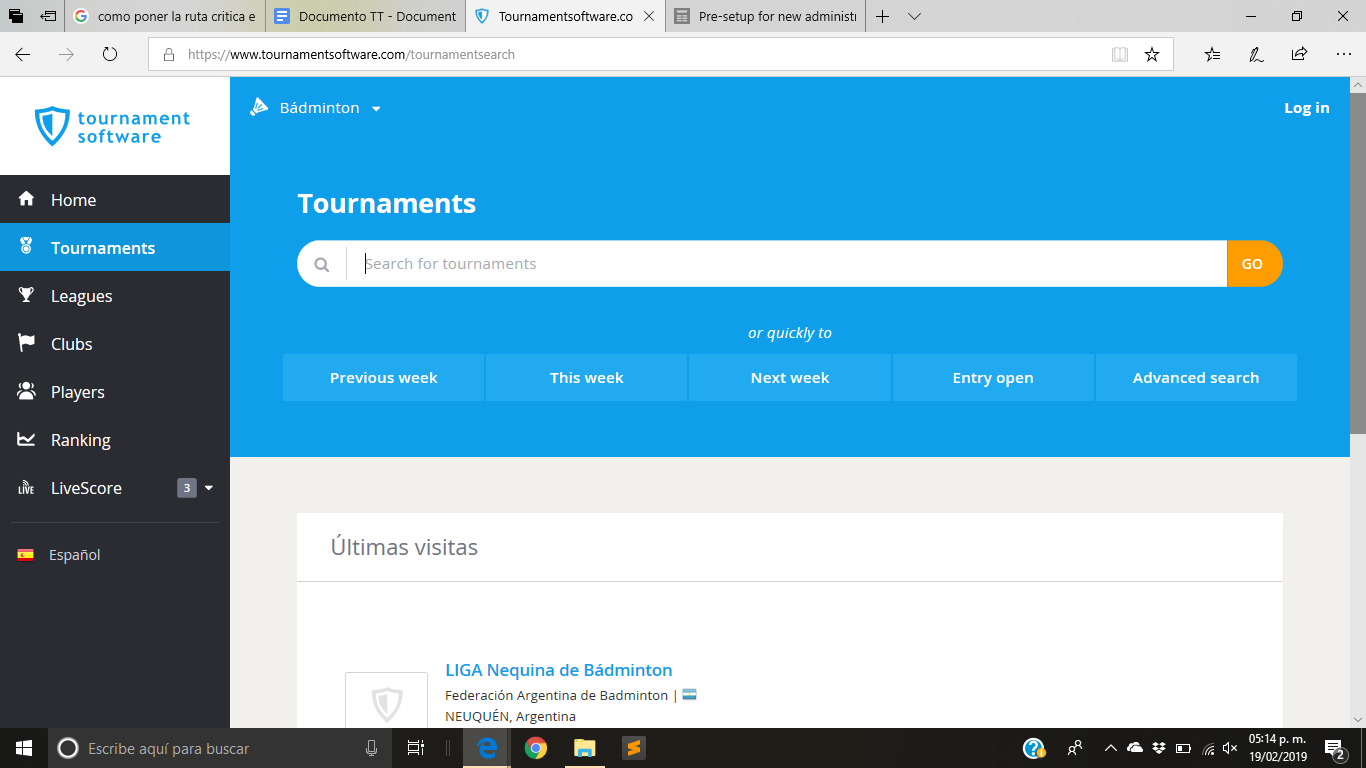
\includegraphics[width=12cm, height=6cm]{Imagenes/Aplicaciones/ToS1.png}
	\caption{Eventos registrados}
\end{figure}
\begin{figure}[h]
	\centering
	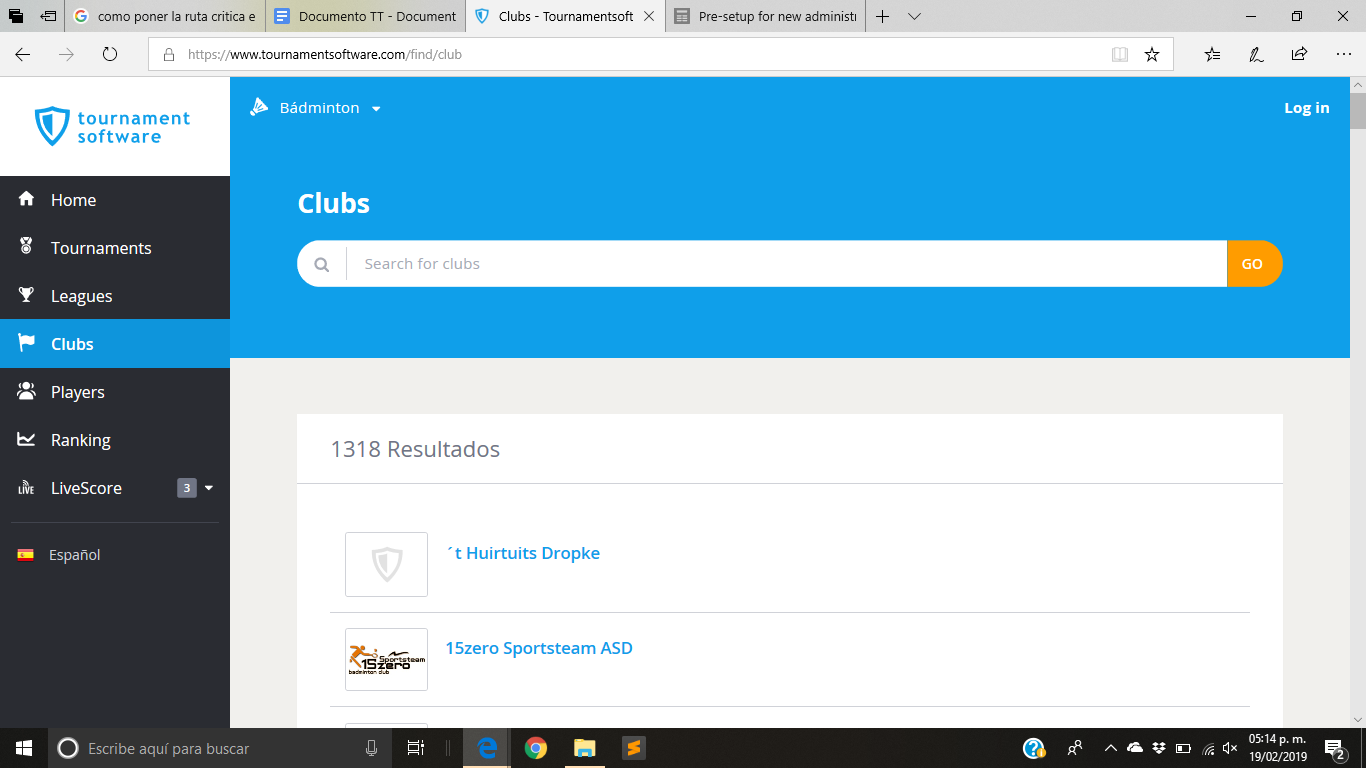
\includegraphics[width=12cm, height=6cm]{Imagenes/Aplicaciones/ToS2.png}
	\caption{Clubs registrados}
\end{figure}
\pagebreak
\begin{figure}[h]
	\centering
	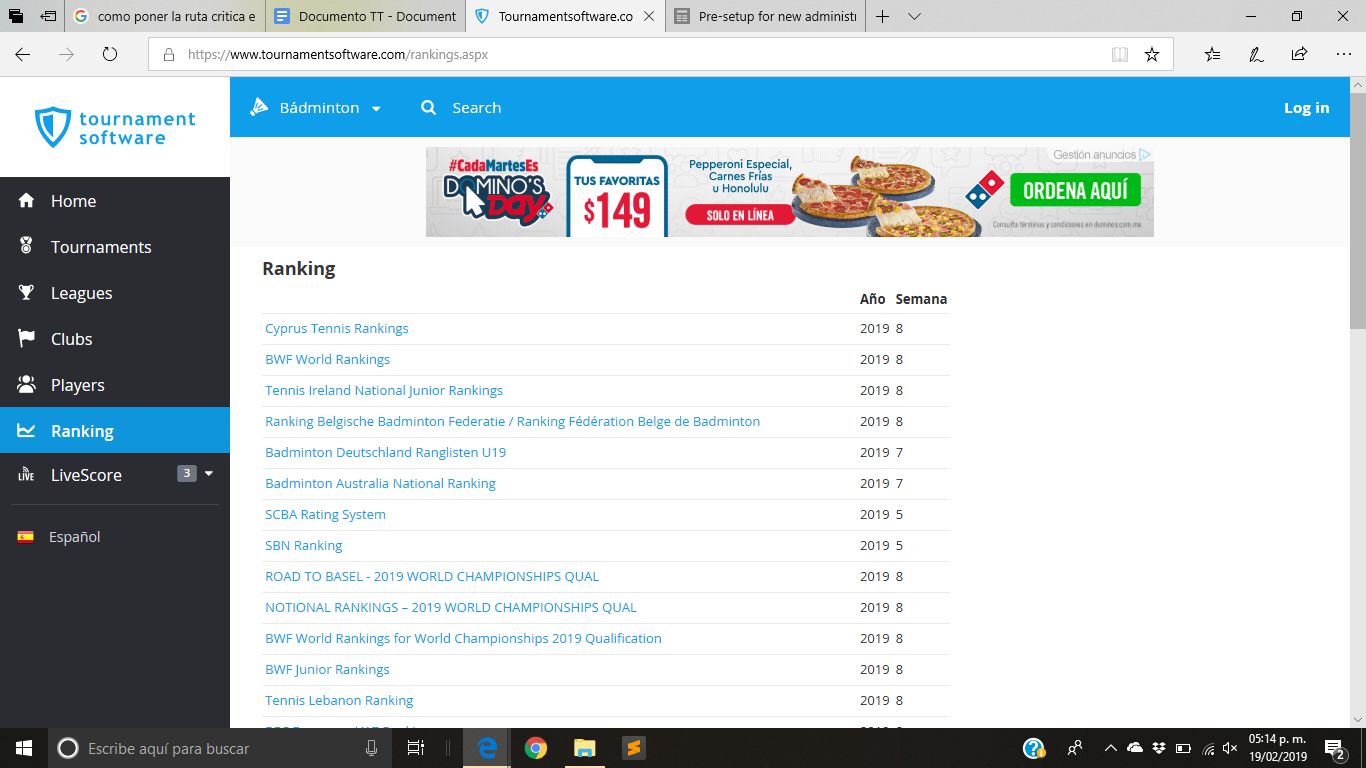
\includegraphics[width=12cm, height=6cm]{Imagenes/Aplicaciones/Tos3.png}
	\caption{Resultados}
\end{figure}

\subsection{Aplicaciones Active Network}
\noindent Esta aplicación ofrece a los usuarios de un manera organizada y fácil, el controlar alguna actividad deportiva, a su vez tienen un mercado más amplio ya que ofrecen sus servicio a escuelas, eventos deportivos, entre otros. Una desventaja que se encontró, es que para cada actividad deportiva se tiene una página designada, que es independiente al resto. \cite{act}
Características: 
\begin{itemize}
	\item Login: Necesario para poder registrar, crear eventos.
	\item Calendario: Muestra los eventos próximos previamente registrados.
	\item Registro de equipos: Permite dar de alta equipos.
	\item Reportes: Generar reportes al final de los eventos.
	\item Registro de eventos: Crea eventos que involucran a los equipos registraos.
\end{itemize}
%=========================================================
%                                                         Imagenes
%=========================================================
\begin{figure}[ht]
	\centering
	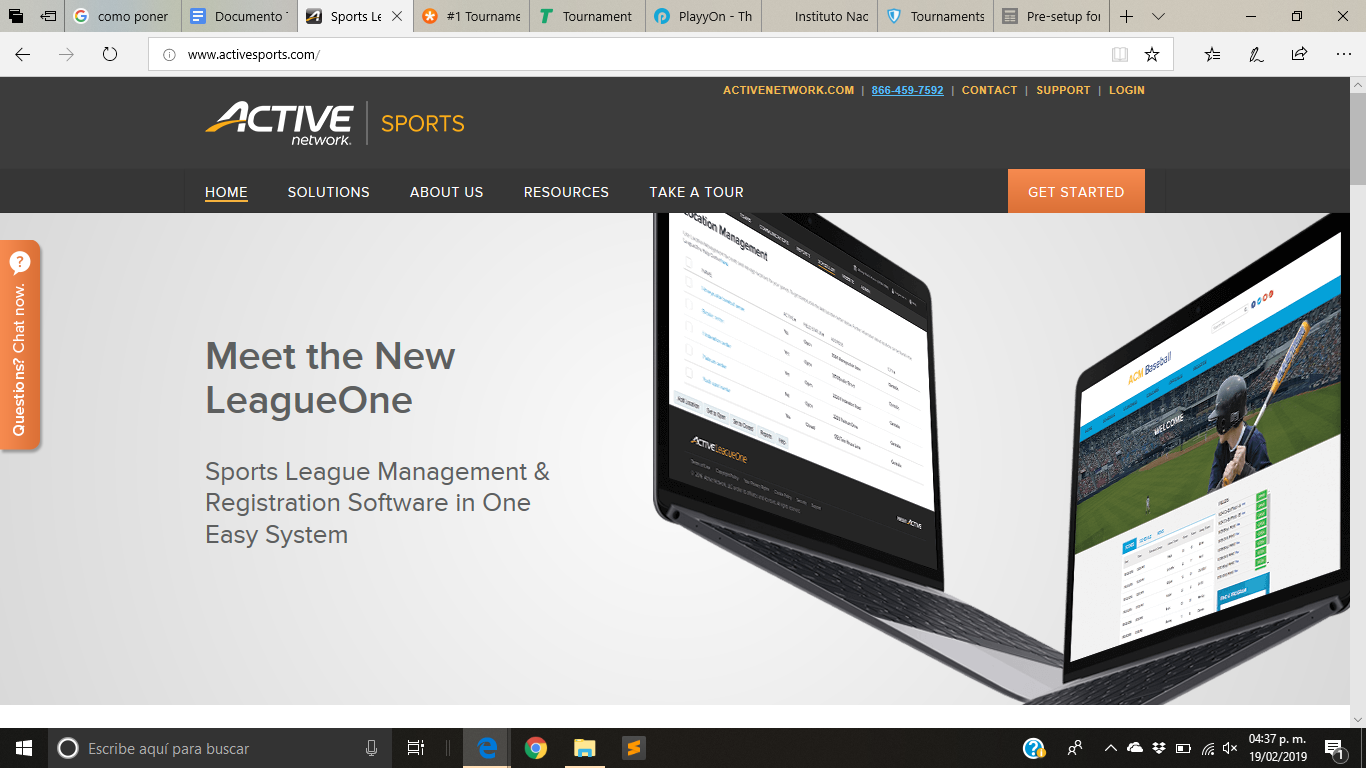
\includegraphics[width=12cm, height=6cm]{Imagenes/Aplicaciones/AN1.png}
	\caption{Página principal}
\end{figure}

\pagebreak

\begin{figure}[ht]
	\centering
	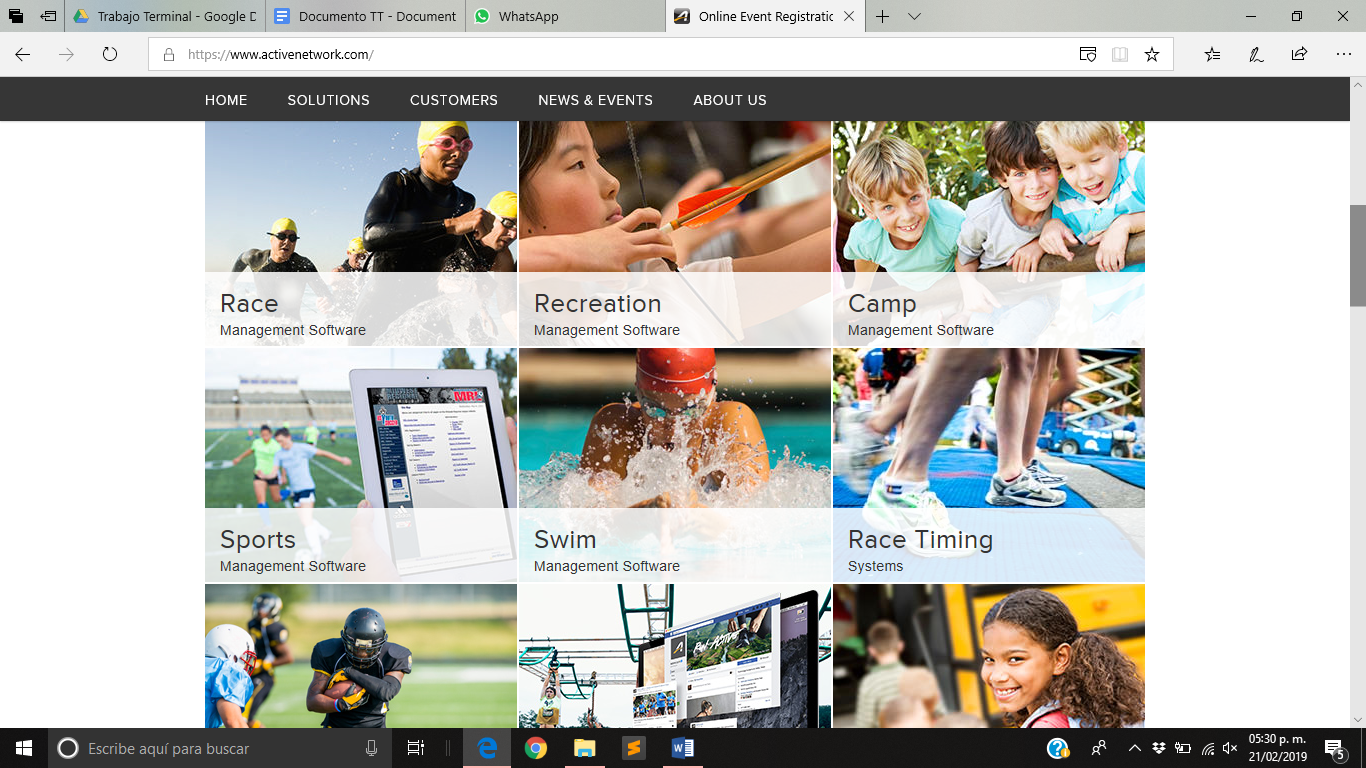
\includegraphics[width=12cm, height=6cm]{Imagenes/Aplicaciones/AN2.png}
	\caption{Eventos deportivos}
\end{figure}


\subsection{Aplicaciones TeamSnap Tournament}
\noindent La aplicación ofrece a los usuarios, un espacio en donde pueden registrar eventos deportivos, agendar o llevar control en el calendario de eventos, saber tablas de posiciones (estadísticas), otra característica de esta aplicación es que tiene un apartado en donde el administrador puede definir el precio de la inscripción a los eventos. \cite{team}
Características: 
\begin{itemize}
	\item Creación de eventos: Generar eventos para que posteriormente los interesados puedan inscribirse.
	\item Dar precio para inscripción a un evento: Permite asignar un monto monetario, si asi se desea para la inscripción a un evento.
	\item Cédula de inscripción: Permite generar el formato de inscripción para los distintos eventos.
	\item Difusión: Una vez creado un evento, se permite promocionar el evento dentro de la misma página.
\end{itemize}
%=========================================================
%                                                         Imagenes
%=========================================================
\begin{figure}[hbt]
	\centering
	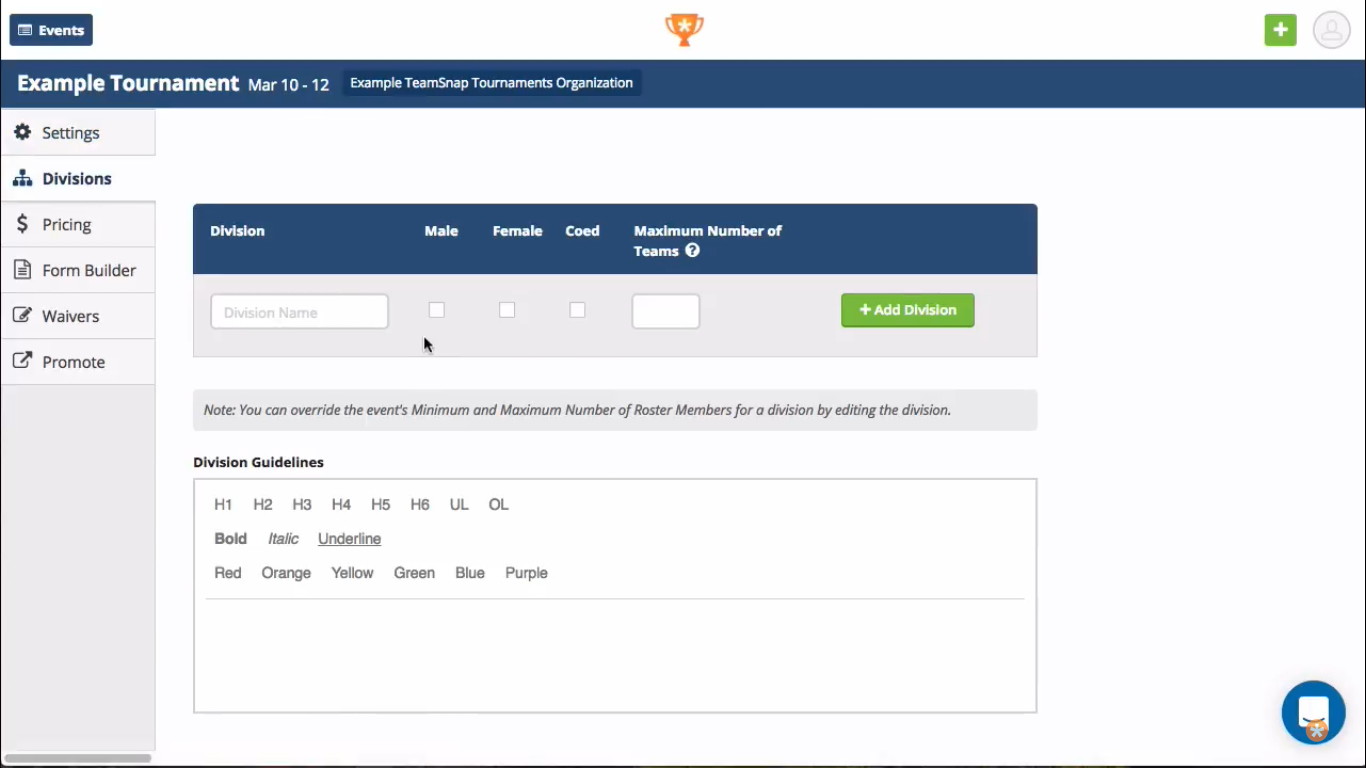
\includegraphics[width=12cm, height=6cm]{Imagenes/Aplicaciones/TsT1.png}
	\caption{Registro de competencias}
		\label{Imagen}
\end{figure}
\pagebreak
\begin{figure}[hbt]
	\centering
	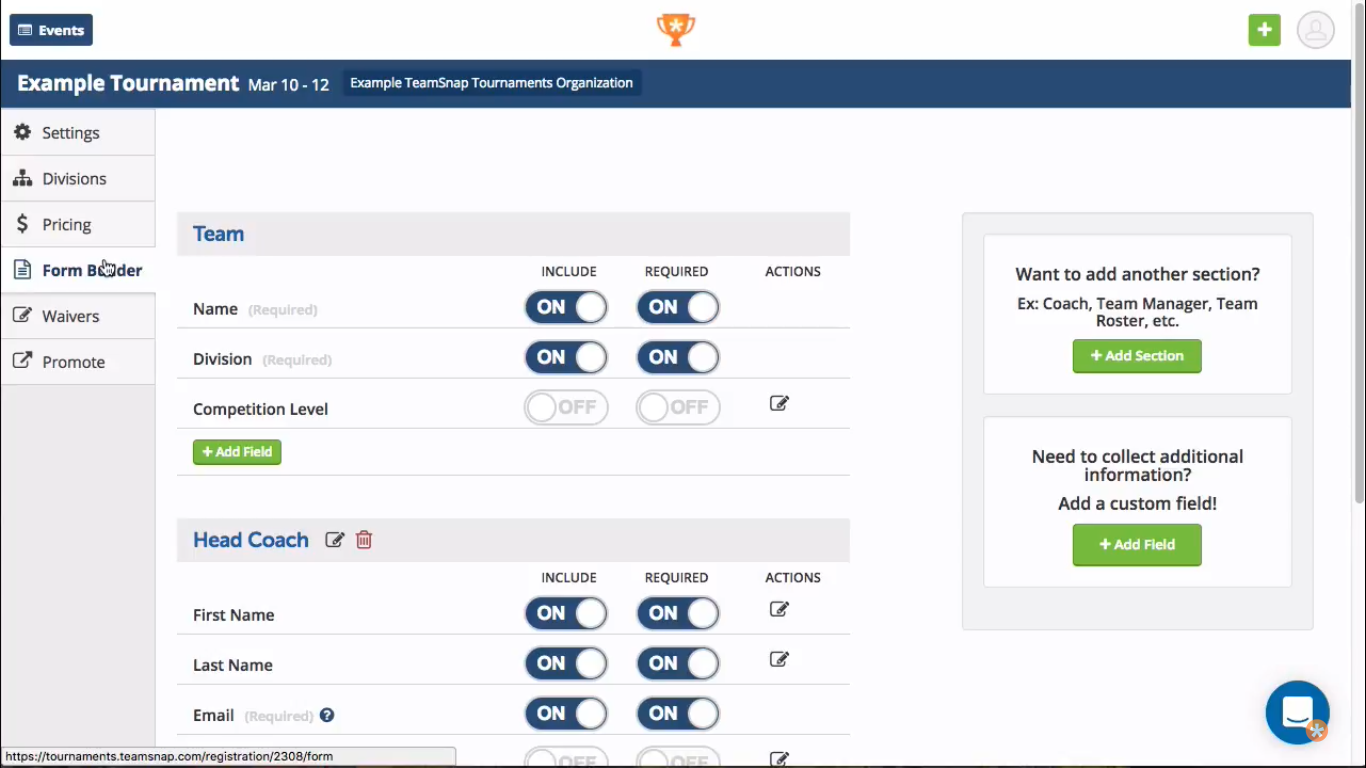
\includegraphics[width=12cm, height=6cm]{Imagenes/Aplicaciones/TsT2.png}
	\caption{Creación de cédula de inscripción}
\end{figure}
\begin{figure}[hbt]
	\centering
	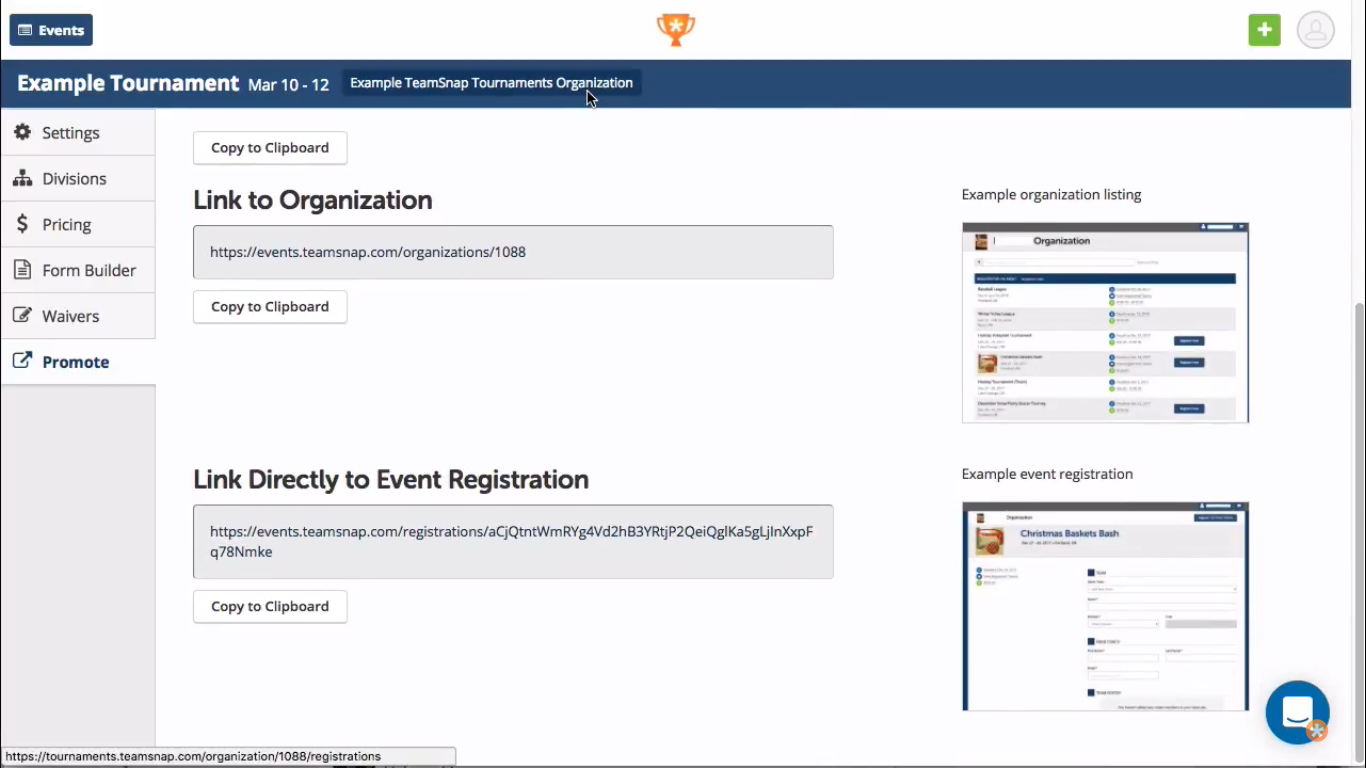
\includegraphics[width=12cm, height=6cm]{Imagenes/Aplicaciones/TsT3.png}
	\caption{Promover}
\end{figure}
\pagebreak


\subsection{Aplicaciones TorneoPal}
\noindent Esta aplicación, al igual que las anteriores, ofrece a los usuarios el generar un horario de actividades, generar torneos entre los equipos registrados y a su vez, en el apartado de estadísticas, ver en una tabla general el estatus de los equipos. \cite{tp}
Características: 
\begin{itemize}
	\item Creación de eventos: Permite crear eventos y asignar, si lo desea un límite de edad para los participantes, el número máximo de integrantes por equipo entre otras características.
	\item Resultados: Una vez concluido los eventos se puede ingresar los resultados para que puedan ser visualizados.
	\item Eliminar eventos: En caso de que se desee, se puede eliminar un evento.
	\item Cambio de equipo en categorías: Se puede modificar un evento, en este caso modificar la categoría en la que se participará.
	\item Informe a árbitros: Se le informa al personal de árbitraje de los eventos que han sido asignados.
	\item Calendario: Muestra los eventos próximos registrados.
	
\end{itemize}
%=========================================================
%                                                         Imagenes
%=========================================================
\begin{figure}[h!]
	\centering
	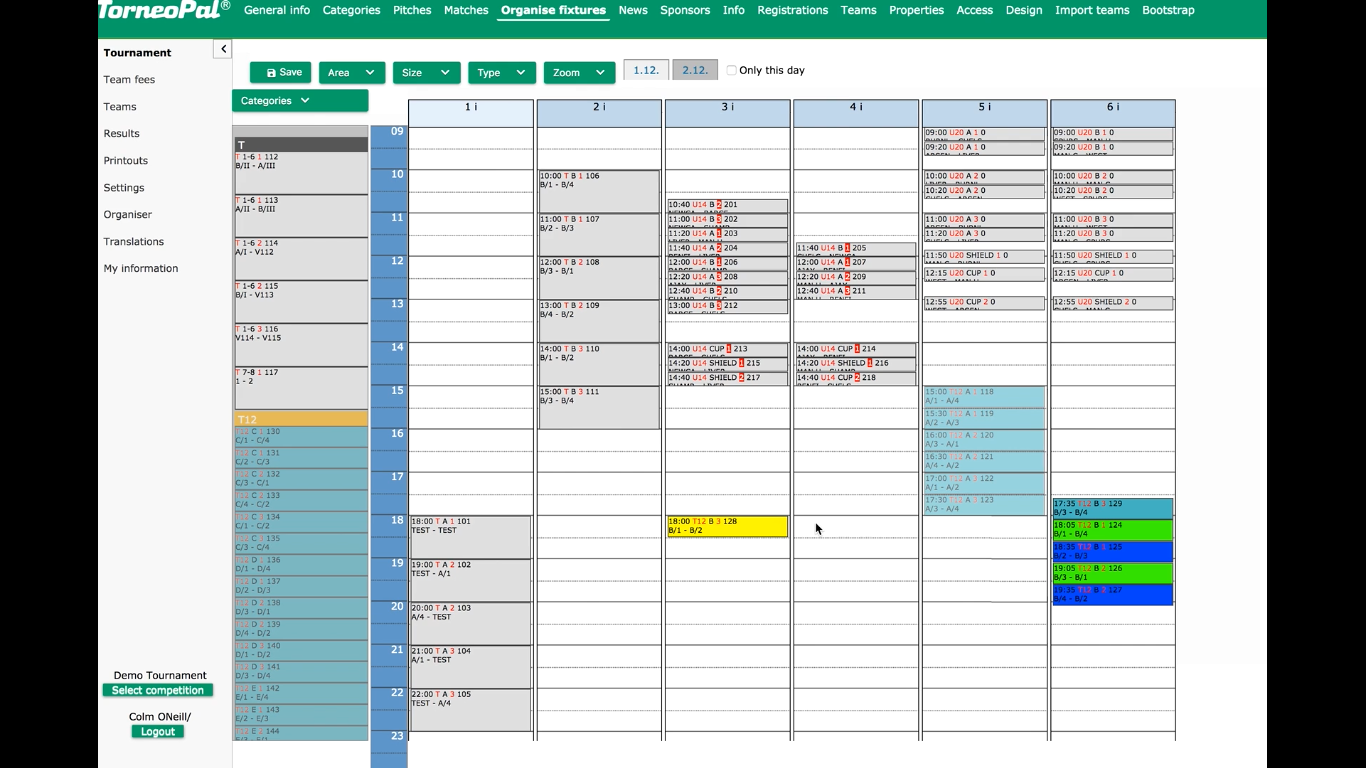
\includegraphics[width=12cm, height=6cm]{Imagenes/Aplicaciones/TP1.png}
	\caption{Calendario de eventos}
\end{figure}
\begin{figure}[h!]
	\centering
	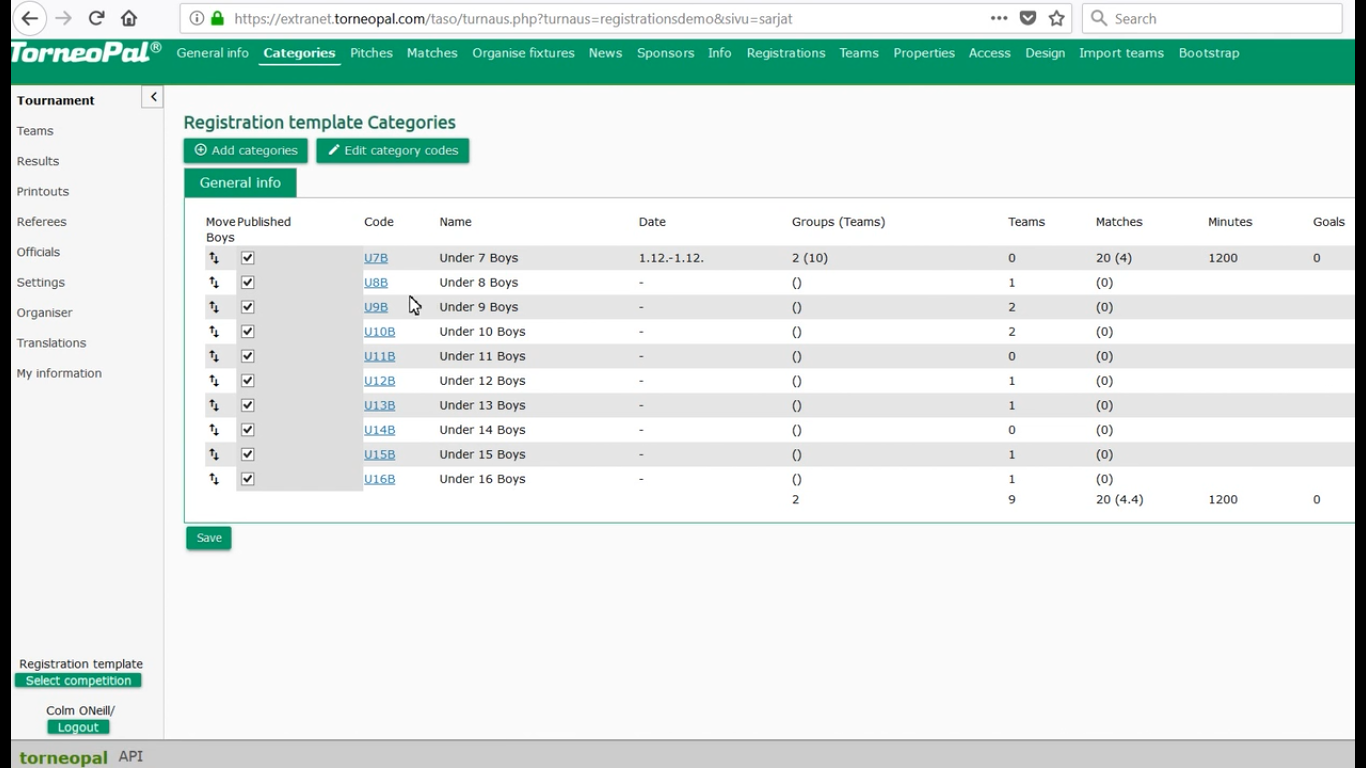
\includegraphics[width=12cm, height=6cm]{Imagenes/Aplicaciones/TP2.png}
	\caption{Registro eventos}
\end{figure}
\pagebreak

\subsection{Aplicaciones Instituto Nacional del deporte CHILE}
\noindent Esta aplicación está dirigida a un mercado en específico, ofreciendo dentro de esta un calendario de próximos eventos, registrarse en alguno del interés del usuario, como complemento se informa los requisitos para poder participar en los eventos y  un apartado en donde pueden dar de alta a organizaciones. No cuenta con un apartado donde muestre estadísticas. \cite{IND}
Características: 
\begin{itemize}
	\item Registro: Dirigido a los estudiantes que deseen participar en los eventos ya registrados.
	\item Calendario: Muestra de manera general los eventos próximos.
	\item Informes: Proporciona información general a los interesados.
	
\end{itemize}
%=========================================================
%                                                         Imagenes
%=========================================================
\begin{figure}[hbt!]
	\centering
	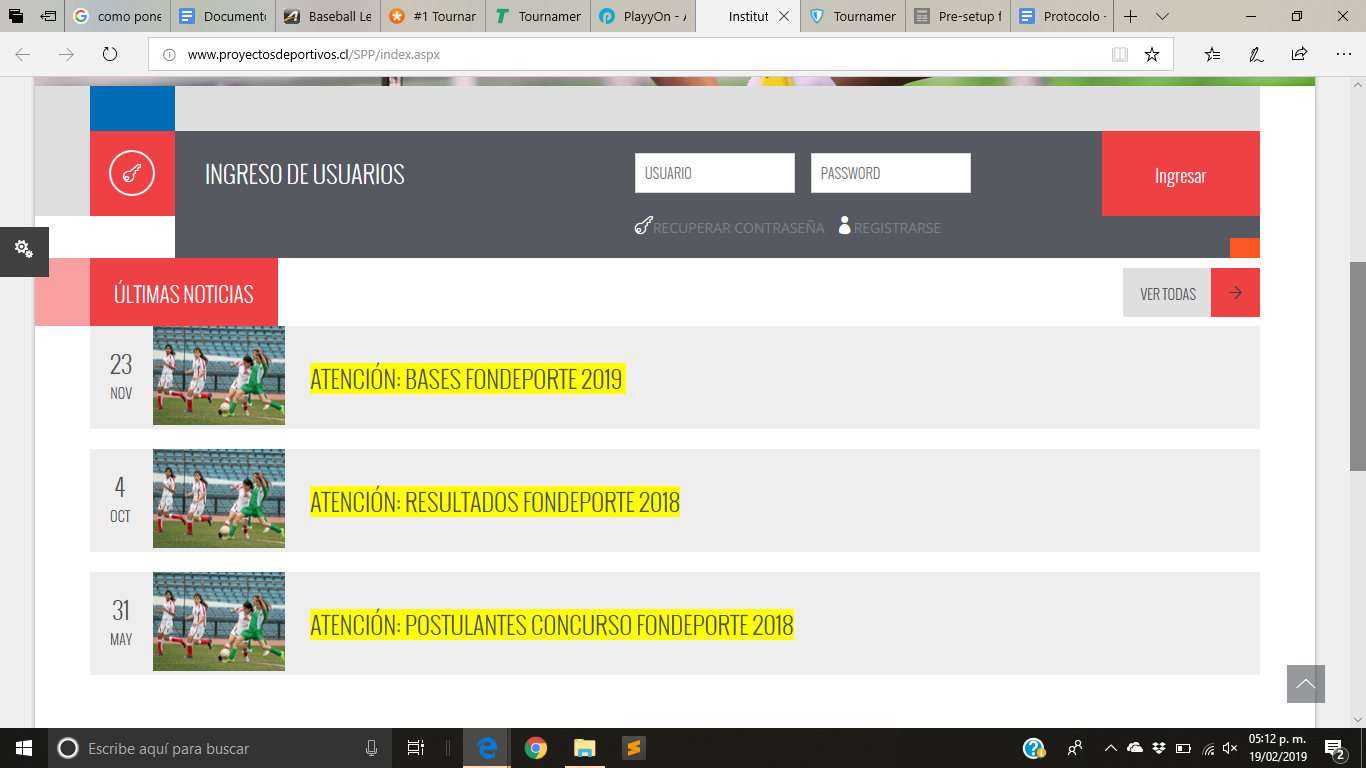
\includegraphics[width=12cm, height=6cm]{Imagenes/Aplicaciones/INDC1.png}
	\caption{Calendario de eventos}
\end{figure}
\begin{figure}[hbt!]
	\centering
	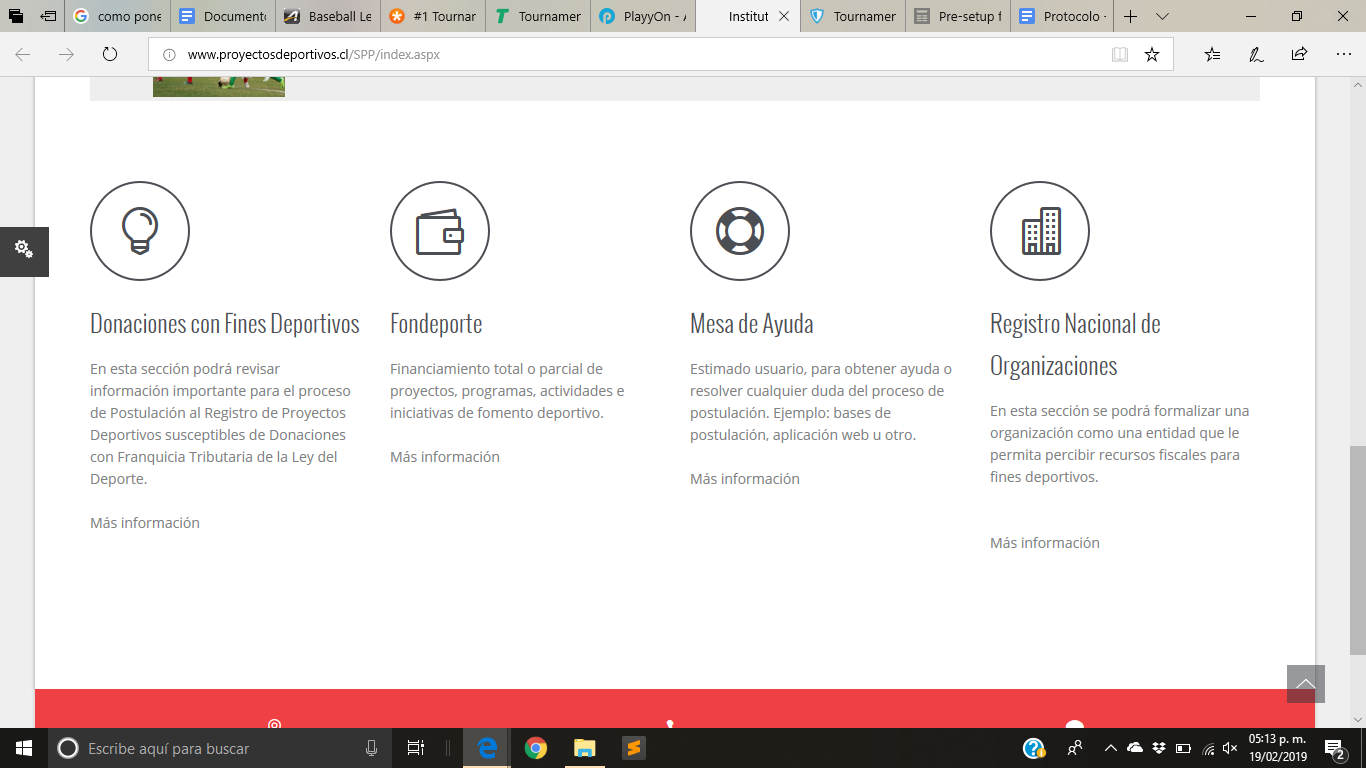
\includegraphics[width=12cm, height=6cm]{Imagenes/Aplicaciones/INDC2.png}
	\caption{Contacto}
\end{figure}
\pagebreak

\subsection{Prototipo para el registro a interpolitécnicos RIDESCOM}
\noindent Esta aplicación esta dirigida a la comunidad del Instituto Politécnico Nacional, especificamente en la Escuela Superior de Cómputo. La cual ofrece a la comunidad un espacio donde pueda ver el calendario de eventos próximos, resultados de la comunidad que participó, así como la posibilidad de inscribirse a un evento cuando estos esten disponibles. 
\\Dentro de la investigación se encontró características en común en todas las aplicaciones, que para nuestro caso en particular ayuda a atacar la problemática, sin embargo ninguna de ellas cumple con todos los requisitos que se busca, ya sea porque no cumple con todos los puntos o en algunos casos, es necesario realizar una subscripción para poder hacer uso del servicio que se ofrece. Sin embargo se puede tomar como punto de referencia algunos casos para ser implementados en nuestra aplicación.
Las características que pretende tener nuestro proyecto son las siguientes:
\begin{itemize}
	\item Registro de eventos: Crear eventos deportivos para que los interesados puedan inscribirse en estos.
	\item Calendario de eventos: Se mostrará los eventos que ya han sido registrados.
	\item Resultados: Una vez que se concluyan los eventos, podrán ingresar los resultados de los participantes para que pueda ser vistos por la comunidad escolar.
	\item Inscripción a eventos: Permitir a los alumnos interesados inscribirse en el evento de su interes. 
\end{itemize}

\noindent A continuación se muestra una tabla comparativa, en la que se muestran las caracteristicas de las aplicaciones antes mencionadas y el proyecto propuesto. Para más detalles consulte la \ref{tablacomparativa}.

\begin{figure} [hbt!]
	\centering
	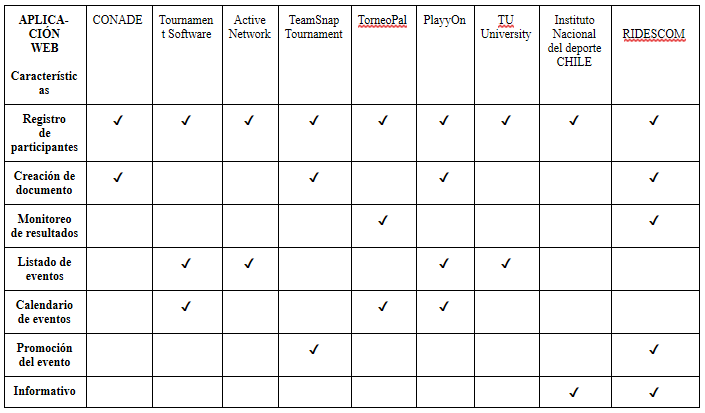
\includegraphics[width=15cm, height=6cm]{Imagenes/tablaComparativa}
	\caption{Caracteristicas principales de las páginas similares.}
	\label{tablacomparativa}
\end{figure}

\noindent El problema que resuelve el trabajo terminal es: la inscripción de personas ajenas al Instituto Politécnico Nacional, la comprobación del estatus académico de los participantes con base ene el reglamento que propuso el Departamento de Fomento Deportivo.